\documentclass{article}
\usepackage{graphicx}
\usepackage{float}
\usepackage[utf8]{inputenc}
\title{The Importance of Elasticity in a Computing Cluster}
\date{}
\author{Marcel Stolin \\ marcelstolin@gmail.com}

\begin{document}


\maketitle


\begin{abstract}
Since the beginning of Big Data, batch processing was the most popular choice for processing large amounts of generated data. These existing processing technologies are not suitable to process the large amount of data we face today. Research works developed a variety of technologies that focus on stream processing. Stream processing technologies bring significant performance improvements and new opportunities to handle Big Data. In this paper, we discuss the differences of batch and stream processing and we explore existing batch and stream processing technologies. We also explain the new possibilities that stream processing make possible.
\end{abstract}


% ==============================
% ###############################
% ==============================
\section{Introduction} \label{s_intro}


% ==============================
% ###############################
% ==============================
\section{Related Work} \label{s_related}


% ==============================
% ###############################
% ==============================
\section{Elasticity} \label{s_batch}

\begin{figure}[h!]
  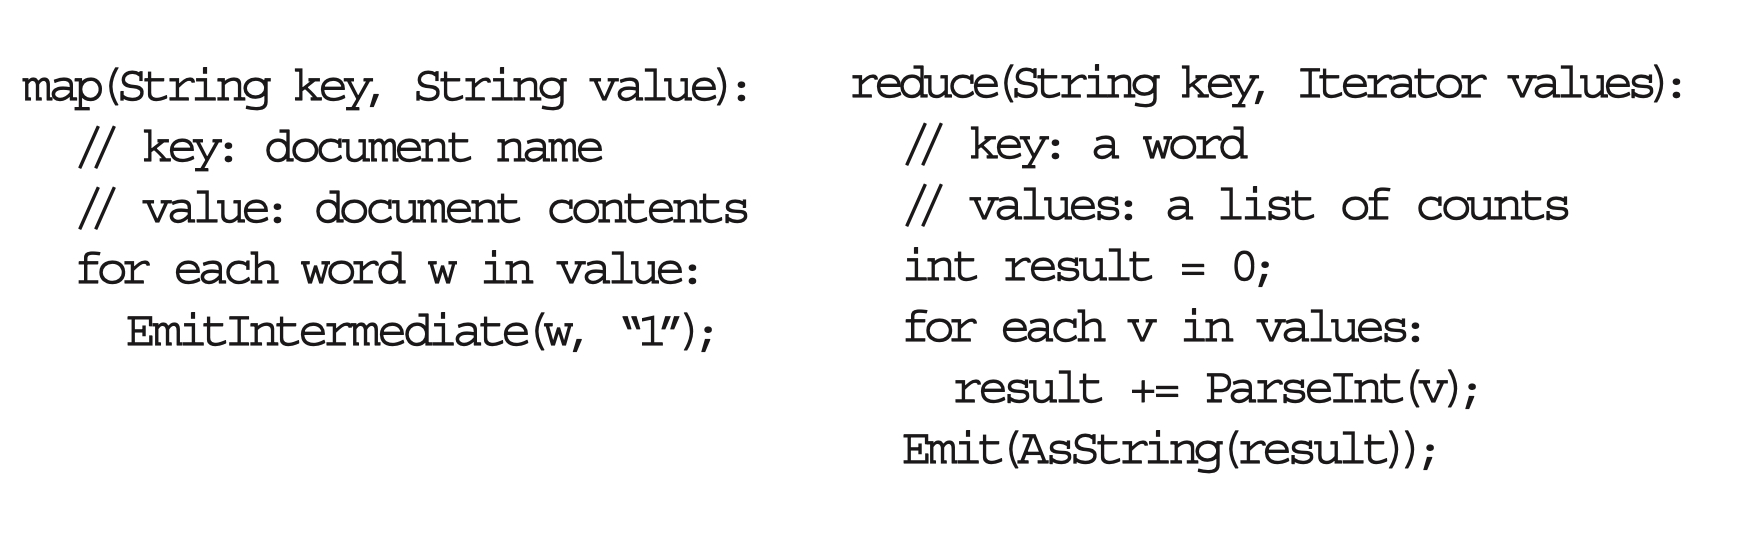
\includegraphics[width=\linewidth]{images/mapreduce.jpg}
  \caption{Pseudo code of counting the number of occurrences of each word in a large selection of documents.}
  \label{fig:mapreduce}
\end{figure}


% ==============================
% ###############################
% ==============================
\section{Design} \label{s_stream}


% ==============================
% ###############################
% ==============================
\section{Conclusion}\label{s_concl}

This paper explains the two data analysis concepts batch processing and stream processing. Since realtime analysis is needed to face the issues of today's demands, batch processing is still being used for legacy implementations and data analysis where no efficient algorithms are known. Stream processing offers new opportunities to handle big data and response with an immediate result to the user.


% ==============================
% ###############################
% ==============================
\bibliographystyle{plain}
\bibliography{mybib}

\end{document}